\documentclass[conference]{IEEEtran}
\IEEEoverridecommandlockouts
% The preceding line is only needed to identify funding in the first footnote. If that is unneeded, please comment it out.
\usepackage{cite}
\usepackage{amsmath,amssymb,amsfonts}
\usepackage{algorithmic}
\usepackage{enumitem}
\usepackage{graphicx}
\usepackage{textcomp}
\usepackage{xcolor}
\def\BibTeX{{\rm B\kern-.05em{\sc i\kern-.025em b}\kern-.08em
    T\kern-.1667em\lower.7ex\hbox{E}\kern-.125emX}}
\graphicspath{{Figures/}}
\usepackage[normalem]{ulem}

\begin{document}

\title{Secure Industrial Control System with Intrusion Detection\\
% {\footnotesize \textsuperscript{*}Note: Sub-titles are not captured in Xplore and
% should not be used}
}

\author{\IEEEauthorblockN{M Rayhan Ahmed Mithu, Rajesh Manicavasagam}
\IEEEauthorblockA{\textit{Computer Science Department} \\
\textit{Tennessee Technological University}\\
Cookeville, TN, United States of America \\
mmithu42, rmanicava42@students.tntech.edu}
\and
\IEEEauthorblockN{Michael Rogers, Denis Ulybyshev}
\IEEEauthorblockA{\textit{Computer Science Department, CEROC} \\
\textit{Tennessee Technological University}\\
Cookeville, TN, United States of America \\
mrogers, dulybyshev@tntech.edu}
% \IEEEauthorblockN{3\textsuperscript{rd} Given Name Surname}
% \IEEEauthorblockA{\textit{dept. name of organization (of Aff.)} \\
% \textit{name of organization (of Aff.)}\\
% City, Country \\
% email address}
% \and
% \IEEEauthorblockN{4\textsuperscript{th} Given Name Surname}
% \IEEEauthorblockA{\textit{dept. name of organization (of Aff.)} \\
% \textit{name of organization (of Aff.)}\\
% City, Country \\
% email address}
% \and
% \IEEEauthorblockN{5\textsuperscript{th} Given Name Surname}
% \IEEEauthorblockA{\textit{dept. name of organization (of Aff.)} \\
% \textit{name of organization (of Aff.)}\\
% City, Country \\
% email address}
% \and
% \IEEEauthorblockN{6\textsuperscript{th} Given Name Surname}
% \IEEEauthorblockA{\textit{dept. name of organization (of Aff.)} \\
% \textit{name of organization (of Aff.)}\\
% City, Country \\
% email address}
}

\maketitle

\begin{abstract}
Security breaches in Industrial Control Systems may have a significant impact on human lives and may cause significant financial loss. For that reason, Detecting intrusions and anomalies in Industrial Control Systems at early stages is important to prevent process failure. Detection of intrusion based on network data alone might not be sufficient. Operator error, device or equipment failure, and other non-network events could lead to a critical state. As a result, these events can indirectly lead to anomalous network traffic, and thus the number of false positives and false negatives generated by the intrusion detection system rises. In this paper, we propose a novel approach of using device state information, stored in a secure data container, to improve the detection accuracy. Our methodology allows to detect anomalies as well as their root causes.  
To detect a root cause of an anomaly, providing confidentiality and integrity for device state, which we record as log records, is essential. In this paper, we also present a secure data container that is used to protect log records for devices in cyber-physical systems. Data protection is provided in transit and at rest. Our data container supports role-based and attribute-based access control, so that every party can access only those data subsets for which the party is authorized. Furthermore, we address the insider threat by detecting several types of data leakages that can be made by malicious authorized insiders. 
\end{abstract}

\begin{IEEEkeywords}
intrusion detection, data privacy, industrial control systems, SCADA systems 
\end{IEEEkeywords}

\section{Introduction}
Industrial Control System (ICS) is the technology used to automate the manufacturing process. It is responsible for controlling and managing large number of field devices. The manufacturing industry has seen a huge rise in the adoption of ICS in recent years. The fierce competition among the companies has been the main catalyst for this revolution in the manufacturing industry. According to the study report published by  Market Research Future (MRFR), the industrial control system market will be growing even more in the future~\cite{c1}. A lot of these industrial control systems are deployed in critical infrastructures such as the smart grid, health care systems, water purification, and nuclear plants. As a result, security breaches and attacks can have significant impact on human lives as well as be very costly. Securing these systems has become a priority as a result of the increasing number of attacks in these domain. 
\par Even though many approaches for intrusion detection in ICS are present in the literature, we observe that most of these solutions focus on the network traffic data generated in the ICS. We propose to use device state information along with network data packets to detect intrusions. Consider Figure~\ref{SICSA} which is based on the Purdue Enterprise Reference Architecture~\cite{}. If intrusion is detected in a data network on level 2, we query device at a lower level 1 to check  device state related to the network data that caused intrusion alert on a higher level. Our approach verifies the alert generated by an Intrusion Detection System (IDS) by validating the suspicious network data packet against the device state information. The algorithm verifies whether suspicious network packets that caused the IDS alert is consistent with the state of the lower level devices. Thus, our approach can not only to detect the anomaly, but also find the root cause of the anomaly. 

Device state data is stored as log records in a secure data container, which guarantees confidentiality and integrity of data that is used to detect anomaly root cause. The secure data container provides data protection in transit and at rest. Data along with access control policies are stored in the container in encrypted form. Separate encryption keys, one per data subset, are generated on-the-fly and are not stored inside the container nor on any Trusted Third Party (TTP). The data container supports role-based and attribute-based access control, so that every party can access only those data subsets for which the party is authorized. A Central Authority (CA) is not required for recipient key generation nor for access control policy enforcemen.      
\par The rest of the paper is organized as follows. Section II presents an overview of related work. In Section III the core design of the implementation is presented. Preliminary experimental results are discussed in Section IV. Section V discusses the future work and section VI concludes the paper.  

\section{Related Work}

Concerns over the security of industrial control system has led many researchers to look for various security solutions to protect the network. The following related work focuses on the state of the art of intrusion detection systems (IDS).  The IDS is not only the a popular software-based solution that is in practical use, but also has been a focus of research in securing industrial control systems.

\par Morris, Vaughn, and Dandass~\cite{c2} proposed an intrusion detection system that focuses on devices that are connected with serial link. The authors proposed a Snort-based intrusion detection system for MODBUS RTU/ASCII communication. The MODBUS traffic is converted to MODBUS TCP/IP and sent to Snort for rule matching. Snort was implemented in two setup, one was in passive mode where the traffic is only monitored by Snort and in inline setup includes rules for dropping packets. 
% {\color{red} MDR: Say what they found - what was the result of their research?  Also, it would be good to state its shortcoming as compared to our work.}
A signature based intrusion detection system with state based rules and stand alone IDS rules was presented in a later work in \cite{c9}.
\par A critical state analysis-based intrusion detection approach by Carcano et al. \cite{c4} in SCADA systems uses state information. In this approach the authors defined a language for system description and to represent states of the system. A software virtual image with software object representing all devices of the monitored system was used to monitor the evolution of system states. Critical states were defined with critical formulas. The intrusion detection system was implemented on the virtual image and if the current state was moving towards a critical state an alert was generated.
However, both of the above mentioned approach requires expert domain knowledge to model normal and critical device sate. They also do not address the problem of integrity of the state information from devices which can be attacked. Our approach uses machine learning to identify important device state information and co-relate it with the network packets. Moreover, we use a secure container to store the device state information which provides data privacy and integrity.
\par A multi agent intrusion detection system was proposed by Tsan and Kwong \cite{c3} in industrial network. They implemented the unsupervised Ant Colony Clustering Model (ACCM) in the "decision agent" that is responsible for learning and classification of prepossessed data. This implementation shows the improved performance ant-based clustering. The KDD-Cup99 dataset was used for the test evaluation with different clustering algorithms and feature extraction techniques. K-Means clustering achieves 89.17\% average detection rate and  4.29\% false positive rate with the Fast Independent Component Analysis (FastICA) feature extraction. A false alarm nearly five per cent of the time could lead to disastrous consequences.
% {\color{red} MDR: Here is a good time to make a statement about how such false postitives are high.  .}
% {\color{red} MDR: state what is different from our work.  Example: they need domain experts to model device behavior.  These domain experts need to be experts on how the device hardware works, and also experts on the industrial process to understand how the device state can move toward critical states.  However, our approach will require no such domain expertise, but will use machine learning techniques to associate device state with network patterns.  Also point out that they do not not address the problem of the integrity of the device state, which can also be attacked.  We use secure data containers to ensure device state integrity.}

Ranchal et al \cite{c10} proposed EPICS solution for web services to protect data throughout the service interaction lifecycle. This solution expands the Active Bundle concept [1] for data protection. Data are stored and transferred together with the access control policies and with the data disclosure monitor. Our solution for secure data container expands the Active Bundle concept with the following capabilities:
(a) detection of data leakages that can be made by authorized insiders;
(b) more secure scheme for encryption key generation;
(c) support of data container in the form of Excel file, which provides compatibility with Microsoft Office, used in many corporate IT infrastructures.  
                                                                            
\section{Core Design}
% \subsection{Industrial Control Systems Security}
%%Industrial control system was initially designed to operate within a close environment and manage the overall system. However, this has changed as the ICS network is now globally connected via the internet technology. The global connection has a lot of benefits that includes managing multiple field sites with thousands of devices in different location from one control center, faster data access and and inseparability among devices with different communication protocols. It also exposed the industrial control system to all the vulnerabilities and security threats that exists in the commercial network.Communication among the main components such as programmable logic controller (PLC), supervisory control and data acquisition (SCADA), Control devices is what makes this whole system functional. The communication protocols for these components are not similar to the typical commercial network protocols. Security was not a big concern when these protocols were designed as the system was kept isolated from the outside world. 
Initially, industrial control systems were constructed in a local context.  In other words, processes were controlled locally and had limited access.  However, as processes became more complex and business needs grew, local control and data access became too limiting.  Therefore, to provide wide access to data and control, devices were connected to wide area networks, and eventually, to the the Internet.

Unfortunately, the unlimited access of the Internet made the control systems vulnerable to attacks, and those protocols and device features that were initially designed for controlled local access had little or no security.  Furthermore, retrofitting existing devices with new protocols and security features is often not practical because the devices are low power and cannot implement the security algorithms given their real-time constraints, or would require major rewrites of software or hardware upgrades, which would be prohibitively expensive.

%\begin{figure}[htbp]
%\centering
%\centerline{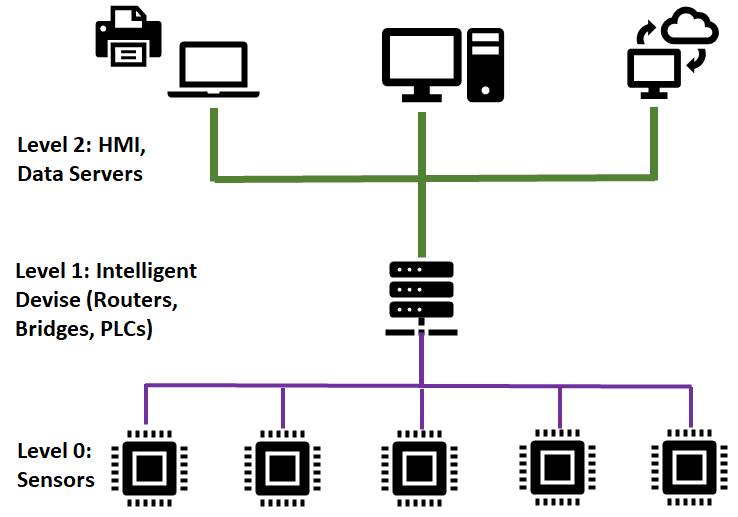
\includegraphics [width=9cm] {ICS-Architecture-RelOK.png}}
%\caption{Industrial Control System Architecture}
%\label{ICS_Arch}
%\end{figure}

Therefore, Intrusion Detection Systems have become a popular security method for detecting attacks.  An IDS can be added to an existing network at a strategic point without needing to modify existing devices.
%Intrusion detection system is a great method for attack detection and prevention in the commercial network by monitoring network traffic with rule based or anomaly based approach. 
However, in the industrial network it is not always enough to just monitor the network traffic. For example, a sequence of (valid) control commands, device failures, faulty raw materials, etc. could lead to a critical situation in the process.  This critical situation will likely result in unusual network traffic as the control devices attempt to notify the process control personnel.   As a result, false positives indicating that the network is being attacked are generated by the IDS.  Believing that a network attack is underway, the process control personnel might not respond correctly to the critical state, which could have disastrous results. 

We propose a novel approach where the IDS can validate network traffic with the help from the device generating the traffic.  Log records of device state information is created and stored. The device state information is kept in a secure container which can be access upon request. Machine learning algorithms will learn what device state is associated with which network communication patterns, and provide this information as a database to the IDS. The IDS will monitor network patterns and, when an anomaly is suspected, can query the secure containers for involved devices, and the database, to validate its suspicions. We call this a secure industrial control system architecture and it is demonstrated in Figure~\ref{SICSA}. 
%%The architecture has four major components:
The architecture has five major components that are described as follows.

%%\begin{enumerate}[label=(\alph*)]
%%\item Offline Tools for Intrusion Detection
%%\item SCADA components
%%\item Secure Container
%%\item Intrusion Detection Process
%%\end{enumerate}
%%\subsection{Offline Tools for Intrusion Detection}

% {\color{red} Ok, so following is what I think we need to describe:  First, all components feed into the secure data container component.  That component provides a secure mechanism for storing and retrieving data for all the other componenents in the system.  The  Embedded component runs on the SCADA devices and collects device state.  It can do this in a miriad of ways, including sampling, logging. etc.  It produces a log file that is stored in a secure data container.  The State identification module uses log records of state stored in a secure container to produce an image that represents an instantaneous state of the system that likely results in a change in network state.  The training component trains  offline.  Its training accomplishes two goals.  One is learning what state information is most likely to result in significant network traffic pattern changes (this information is used by the state identification module), and the other is learning what device state produces particular network state. So, we need to restructure/rewrite the description below to reflect this.  See my simplistic picture:}
% 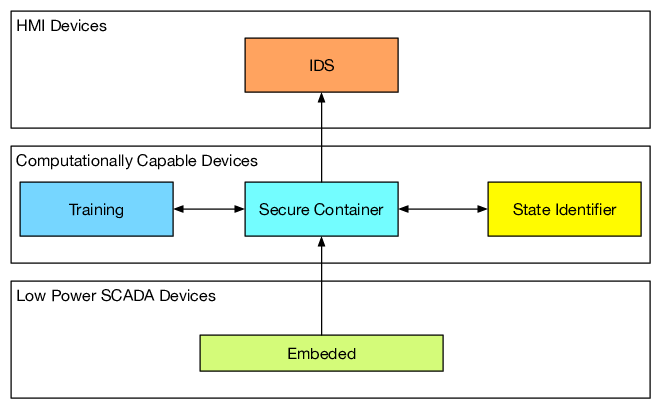
\includegraphics [width=.4\textwidth]{secscada.png}
\begin{figure}[htbp]
\centering
\centerline{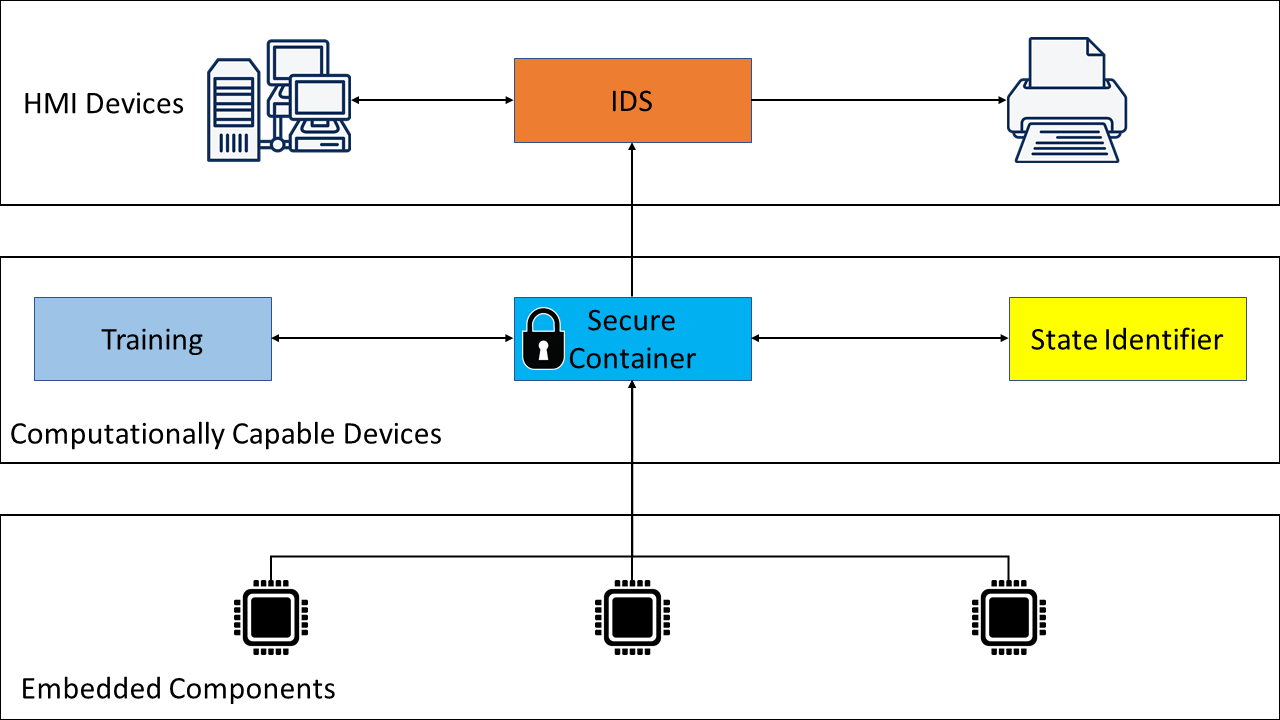
\includegraphics [width=.5\textwidth]{sec_scada.png}}
\caption{Secure SCADA}
\label{Sec_scada}
%
\end{figure}

\subsection{Embedded Components}
The {\em embedded components} of the system will monitor SCADA devices in real time, create log records, and transfer the log records to the secure data container. Two modules are required to execute these actions. The first module is the \textit{\textbf{State Monitor}} and the other module is called \textit{\textbf{State Router}}.

The state monitor module is responsible for real time monitoring of the device state. It can collect device state information in a many of ways, including sampling, logging the .

The device state information collected by the state monitor module will be transferred by the state router module to the secure container. 

%%This node can perform security analysis to identify if the device is compromised.

\subsection{State Identification}
This system component of the architecture is responsible to identify important information about the state of the device. This module uses the information stored in the secure container to produce an image that represents an instantaneous state of the system that likely results in a change of the network data. 

\subsection{Secure Data Container}
Our proposed solution for protecting data in transit and at rest with providing leakage detection, as well as role-based and attribute-based access control, relies on Secure Mobile Protected Agent with Data (SMPAD). The idea was inspired by an Active Bundle concept [2], [3]. SMPAD is a self-protecting data container that incorporates sensitive data in encrypted form with watermarks, access control policies, metadata, provenance data collector, policy and attribute enforcement kernel. SMPAD can be used to store log files as well as sensor data snapshots. Each separate data subset is encrypted with separate encryption key, generated on-the-fly for each client’s role based on the unique information from the SMPAD execution control flow path. The access control model relies on role-based and attribute-based access control model and guarantees that a client will be able to access only those data subsets from a data container for which the client is authorized [4]. Data container provides tamper-resistance and data integrity. Moreover, SMPAD can detect several types of data leakages that can be made by authorized insiders [1]. The novelty of the proposed solution is that it works in both centralized and decentralized peer-to-peer network architectures. Central Authority (CA) is not required neither for data recipient’s key generation nor for access control policy enforcement.

\begin{figure}[htbp]
\centering
\centerline{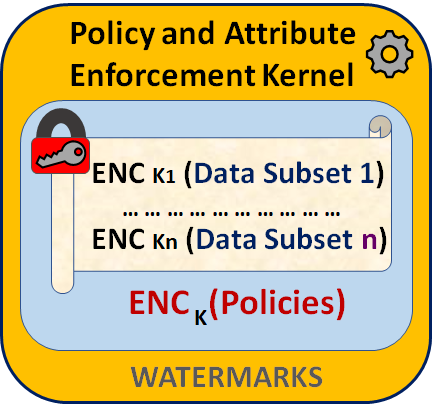
\includegraphics [width=6cm] {SMPAD-RelOK.png}}
\caption{SMPAD: Secure Data Container}
\label{sdc}
\end{figure}

%Denis:
Author in \cite{c6} presents a similar concept, an Extended Attribute-Aware Active Bundle (EA3B). In this paper EA3B concept is improved to make it more secure and to provide easier data container integration into existing software systems. Instead of Java Executable Archive (JAR), data container is being implemented as an Excel table with encrypted worksheets and with Visual Basic macro that enforces access control policies. Using protected Excel table for secure data container makes our solution more compatible with existing software systems. Furthermore, different key generation scheme is applied. Symmetric AES 256 bit key is generated on-the-fly by a Key Derivation Function (KDF) that as an input takes the following parameters: 
(a) hash value of metadata and access control policies 
(b) hash value of VBA macro that enforces policies 
(c) hash value of the X.509 certificate of the Authentication Server (AS)
(d) hash value of a data subset name
Each data subset is stored as a separate worksheet in Excel file with encrypted values. Worksheet is only visible for authorized parties. In contrast with EA3B, there are two ways to access data from data container: 
(1) call API to read value from Excel cell 
(2) open data container in Excel processor, such as Microsoft Office or OpenOffice. 

- list set of supported attributes for ABAC
- talk about data leakage detection via watermarks


\subsection{Training}
We call this component the {\em training module} as these will be executed off-line to train the system such that it learns what device state results in particular network behavior. It will also identify the state information Which are most likely to make significant change in the network traffic. The information form the state identifying module is used here. The training module will be fed data collected from the state collection component and data collected by sampling the network. Machine learning algorithms are used to model the relationship between device state and network traffic and stored in  database. The IDS can query this information to verify its alerts.

 
\subsection{Intrusion Detection Process}
Detection process is the most important component of the secure architecture. This process is responsible for intrusion detection in the SCADA environment. Typical intrusion detection system (IDS) uses the network packets to analyze the traffic and generate alert in case of any abnormal activity in the network. However, in SCADA environment, it is not necessary that an abnormal network behavior will always be the reason for intrusion. Often times a series of valid commands can lead to a critical situation in the SCADA environment that will cause serious damage to the infrastructure. The IDS will not generate any alert in that situation as the network traffic will not look suspicious or abnormal.
\par The intrusion detection system in this component does not rely on only network traffic. If an alert is generated from abnormal activity in the network, IDS can query the information stored by the training module. The relative device state information according to the specific network data is used to verify the alert. This allows the IDS to reduce false positives. The IDS also receives real time information from the state router and performs analysis to detect compromised device. 
\begin{figure}[htbp]
\centering
\centerline{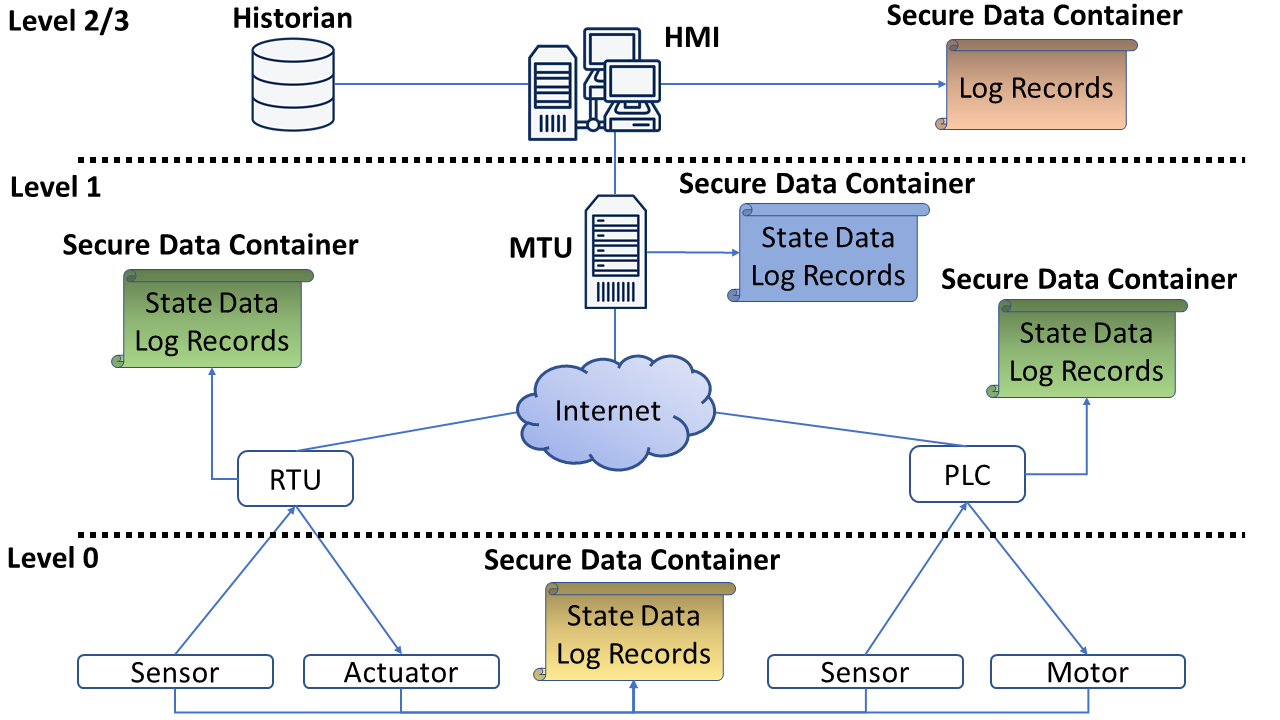
\includegraphics [width=.5\textwidth]{sec_arch.png}}
\caption{Secure Industrial Control System Architecture}
\label{SICSA}
%
\end{figure}

\section{Evaluation}
As a proof of concept that additional device information can help the intrusion detection system, we did a preliminary experiment. We used a dataset \cite{c7} created by the Mississippi State University SCADA Security Laboratory and Power and Energy Research laboratory, which is a collection of network data from a water storage tank system. The dataset is generated for performing intrusion detection to detect seven different attack scenario. it was created for WEKA \cite{c8}, a machine learning tool. Based on the description of the process, we annotated the network trace with data representing sane device state for the network data being generated. We used Naive Bayes algorithm to create a model with the new dataset. The added information helps the machine learning algorithm to increase the true positive rate significantly. This shows that specific information related to network packet can be helpful for machine learning techniques used in intrusion detection. The true positive (TP) rate for attack detection by the algorithm almost doubled. The comparison is shown in Figure ~\ref{eval-anomaly}.
\begin{figure}[htbp]
\centering
\centerline{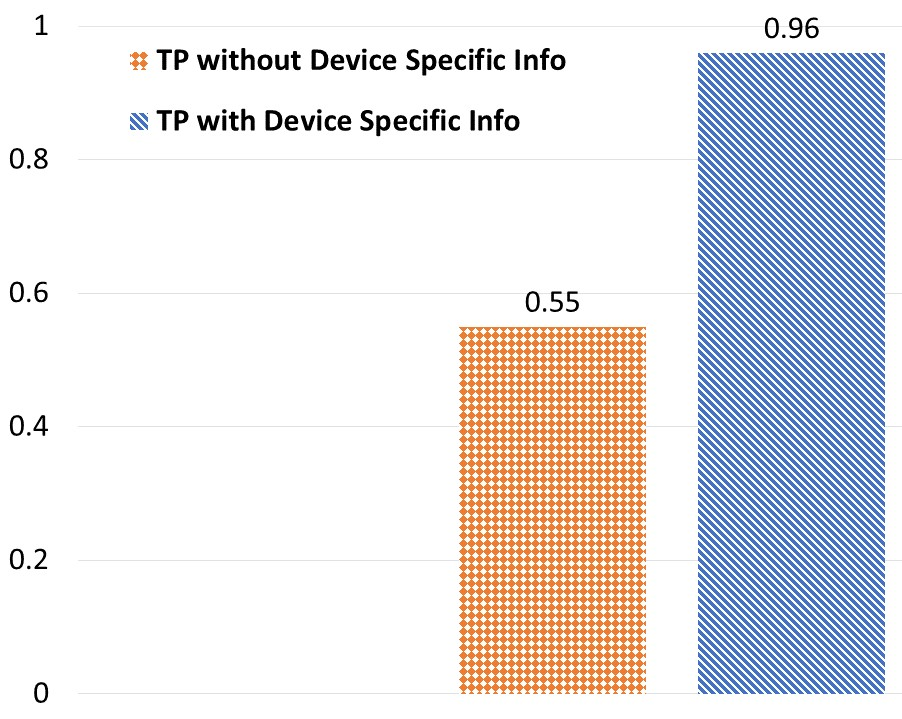
\includegraphics [width=.5\textwidth]{chart.jpg}}
\caption{TP rate for Attack Detection in Water Storage Dataset}
\label{eval-anomaly}
%
\end{figure}
%Denis

Round-trip time for secure data container is measured with ApacheBench utility. 
\begin{center}
\begin{tabular}{ |c|c|c| } 
 \hline
Hardware / Num. of policies & 4 policies & 8 policies \\ 
RPi & 69.51 & 69.67 \\
MacBook & 18.10 & 18.82 \\
 \hline
\end{tabular}
\end{center}

\section{Future Work}
Our future goal is to identify machine learning algorithms to detect important artifacts that are responsible for triggering network data. A dataset will be generated to represent the relationship between the network data and the important device state data. We also plan to determine how to incorporate learned behavior into the intrusion detection system to improve its results and to reduce false positives. Furthermore, we plan to expand secure data container capabilities to provide guarantees for provenance data integrity. We explore blockchain-based approaches for collecting and storing provenance data.   

\section{Conclusion}





\begin{thebibliography}{00}
\bibitem{c1}Industrial Control Systems (ICS) Market 2018 Global Analysis, Industry Size, Share Leaders, Current Status by Major Key vendors and Trends by Forecast to 2023. https://www.marketwatch.com/press-release/industrial-control-systems-ics-market-2018-global-analysis-industry-size-share-leaders-current-status-by-major-key-vendors-and-trends-by-forecast-to-2023-2018-11-29
\bibitem{c2}Morris, T., Vaughn, R., \& Dandass, Y. (2012). A retrofit network intrusion detection system for MODBUS RTU and ASCII industrial control systems. Proceedings of the Annual Hawaii International Conference on System Sciences, 2338–2345. https://doi.org/10.1109/HICSS.2012.78
\bibitem{c3}Tsang, C. H., \& Kwong, S. (2005). Multi-agent intrusion detection system in industrial network using ant colony clustering approach and unsupervised feature extraction. Proceedings of the IEEE International Conference on Industrial Technology, 2005, 51–56. https://doi.org/10.1109/ICIT.2005.1600609
\bibitem{c4}Carcano, A., Coletta, A., Guglielmi, M., Masera, M., Nai Fovino, I., \& Trombetta, A. (2011). A multidimensional critical state analysis for detecting intrusions in SCADA systems. IEEE Transactions on Industrial Informatics, 7(2), 179–186. https://doi.org/10.1109/TII.2010.2099234
\bibitem{c5}Kiss, I., Genge, B., Haller, P., \& Sebestyen, G. (2014). Data clustering-based anomaly detection in industrial control systems. Proceedings - 2014 IEEE 10th International Conference on Intelligent Computer Communication and Processing, ICCP 2014, 275–281. https://doi.org/10.1109/ICCP.2014.6937009
\bibitem{c6} Ulybyshev, Denis A, (2019) "Data Protection in Transit and at Rest with Leakage Detection". Ph.D. Thesis, Purdue University. https://doi.org/10.25394/PGS.8024345.v1
\bibitem{c7}Morris, T. Srivastava, A., Reaves, B., Gao, W., Pavurapu, K., Reddi, R. A Control System Testbed to Validate Critical Infrastructure Protection Concepts. International Journal of Critical Infrastructure Protection (2011). Elseiver. doi:10.1016/j.ijcip.2011.06.005
\bibitem{c8}Eibe Frank, Mark A. Hall, and Ian H. Witten (2016). The WEKA Workbench. Online Appendix for "Data Mining: Practical Machine Learning Tools and Techniques", Morgan Kaufmann, Fourth Edition, 2016.
\bibitem{c9}Gao, W., \& Morris, T. (2014). On Cyber Attacks and Signature Based Intrusion Detection for Modbus Based Industrial Control Systems. Journal of Digital Forensics, Security and Law, 9(1). https://doi.org/10.15394/jdfsl.2014.1162
\bibitem{c10}Ranchal, R., Bhargava, B., Angin, P., \& Othmane, L. B. (2018). Epics: A framework for enforcing security policies in composite web services. IEEE Transactions on Services Computing.

\end{thebibliography}
\vspace{12pt}
\end{document}
